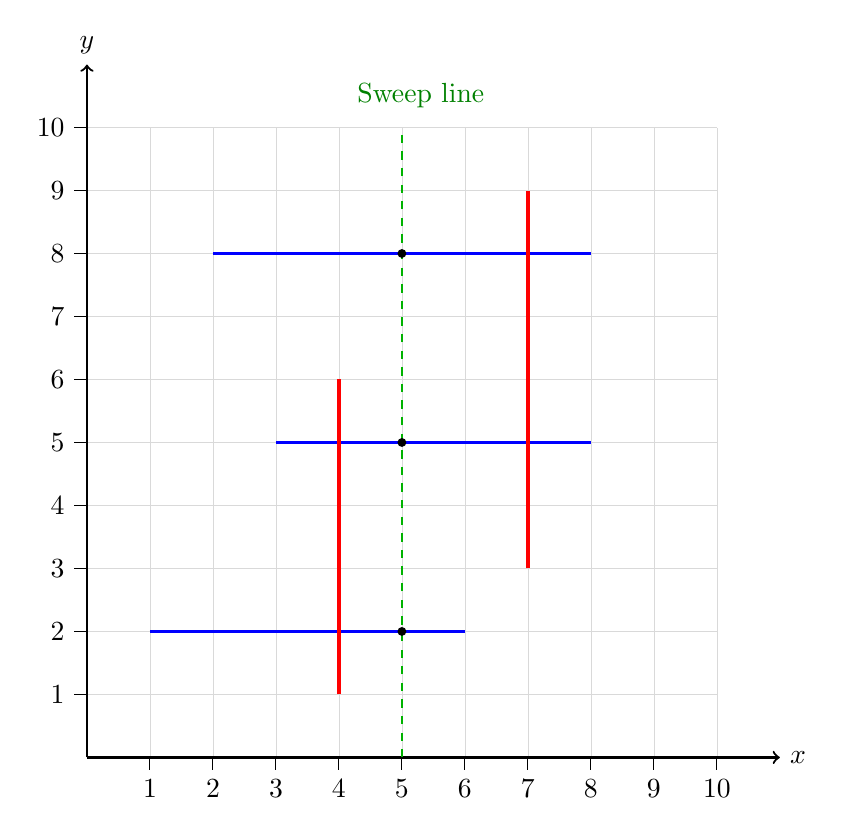
\begin{tikzpicture}[scale=0.8]
    \draw[step=1cm, gray!30, very thin] (0,0) grid (10,10);

    \draw[->, thick] (0,0) -- (11,0) node[right] {$x$};
    \draw[->, thick] (0,0) -- (0,11) node[above] {$y$};

    \foreach \x in {1,...,10}
        \draw (\x,0) -- (\x,-0.2) node[below] {\x};

    \foreach \y in {1,...,10}
        \draw (0,\y) -- (-0.2,\y) node[left] {\y};

    \draw[blue, very thick] (1,2) -- (6,2);
    \draw[blue, very thick] (3,5) -- (8,5);
    \draw[blue, very thick] (2,8) -- (8,8);

    \draw[red, very thick] (4,1) -- (4,6);
    \draw[red, very thick] (7,3) -- (7,9);

    \draw[green!70!black, thick, dashed] (5,0) -- (5,10);
    \node[green!50!black] at (5.3,10.5) {Sweep line};

    \fill[black] (5,2) circle (2pt);
    \fill[black] (5,5) circle (2pt);
    \fill[black] (5,8) circle (2pt);
\end{tikzpicture}